\documentclass[11pt]{article}
\usepackage[margin=0.5in]{geometry}
\usepackage{graphicx}
\usepackage{amsmath}
\usepackage{enumitem}
\usepackage{listings}

\graphicspath{{/home/konner/Documents/Stats_170/HW3/} }
\begin{document}
\centerline{\Large Stats 170 - Time Series Analysis}
\vspace{3pc}
\centerline{\Large Homework 3}
\vspace{.5pc}
\centerline{Konner Macias - 004603916}
\centerline{October 30th, 2018}
\vspace{1.5pc}
\section{}
a. Here we perform the {\tt sqrt} transform on the New Zealand dataset. Here is the updated time plot of 
$$ y_t^\star = \sqrt{y_t} $$
\begin{center}
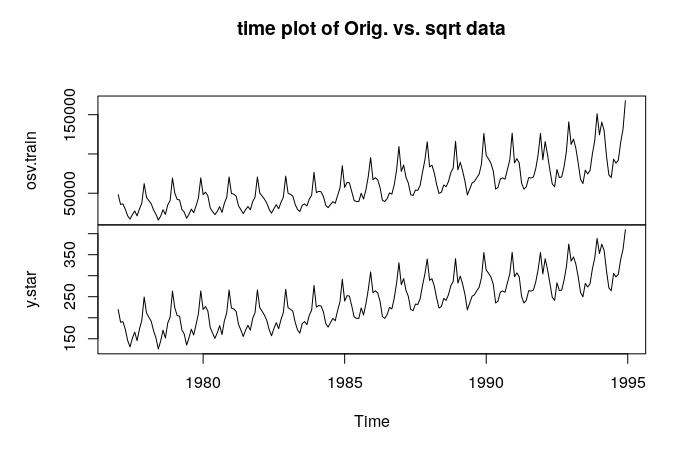
\includegraphics[scale=1]{1a}
\end{center}
We notice that $y_t^\star$, while relatively difficult to notice, does create more of a stationary variance within the data. Looking at both time plots overall, we notice seasonality comparing year to year and also an overall positive upwards trend.
\\\\
b. We notice that the corrrelogram for $y_t^\star$ has all statistically significant lags, but this data is non-stationary so we cannot extract much from this information. The lags appear to rise and fall in a pattern potentially indicating some seasonality. However, we should perform regular differencing first to deal with the obvious trend in the data.
\\\\
c. Here I perform just regular differencing:
\begin{center}
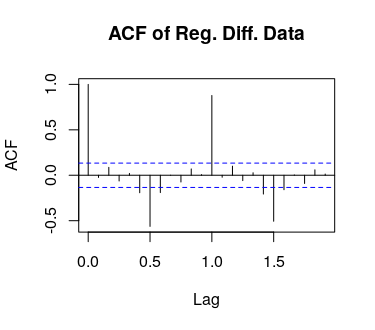
\includegraphics[scale=.8]{1b1}
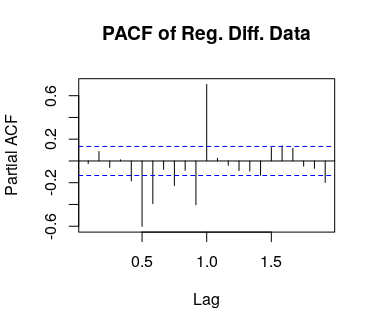
\includegraphics[scale=.8]{1b1a}
\end{center}
Looking at the ACF of just the regularly differenced data, we notice that the data is still not entirely stationary as there are still 3 statistically significant lags, and that we notice possible underlying seasonality through the pattern in the lags.
\\\\
Next we look at the solely seasonally differenced data. 
\begin{center}
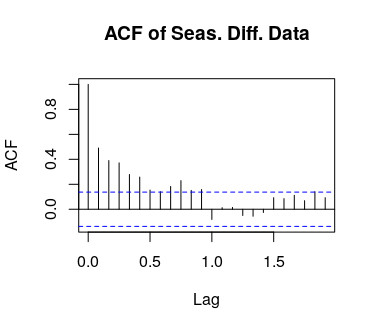
\includegraphics[scale=.8]{1b2}
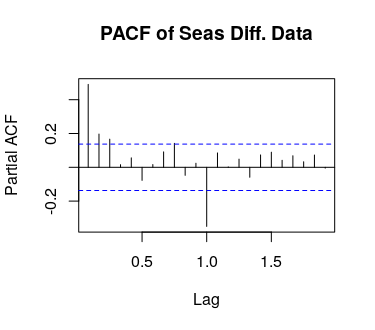
\includegraphics[scale=.8]{1b2a}
\end{center}
Here we still notice that the data isn't entirely stationary yet. There appears to be a slow decay of lags in the ACF from the positive to negative direction, possibly indicating an underlying trend in the data.
\\\\
Next, we look at the seasonally differenced of the regularly differenced data.
\begin{center}
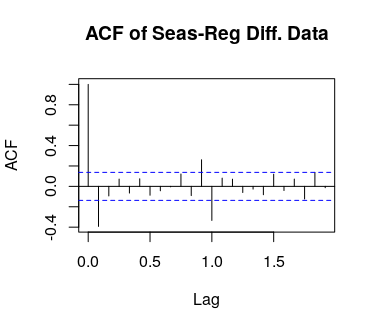
\includegraphics[scale=.8]{1b3}
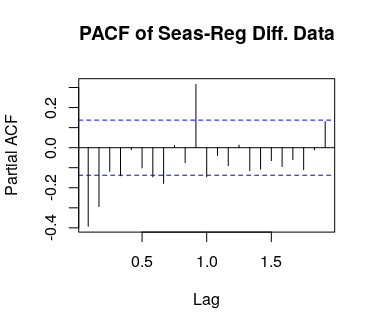
\includegraphics[scale=.8]{1b4}
\end{center}
Compared to the previous ACF's, we notice that seasonally differencing the regularly differenced data proved the most suitable method for making the data stationary. We still notice 2 statistically significant lags, but that is alright as the other statistically significant lag appears to be at the seasonal step in time. We shall call this new data $ y_t^{\star\star} $.
\\\\
d. Here we compare Model 1: $SARIMA(1,1,0)(1,1,0)_1 2$ and Model 2: $SARIMA(0,1,1)(0,1,1)_1 2$ for the squared root data. Below are the ACF's and PACF's of the residuals of each model.
\begin{center}
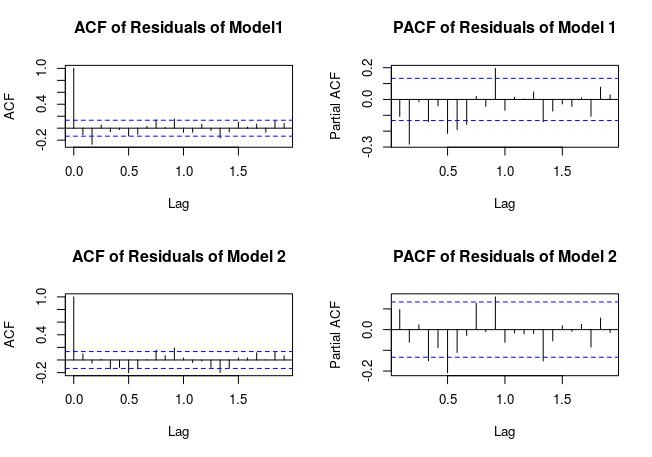
\includegraphics[scale=1]{1d}
\end{center}
Comparing the two models, we notice an early significant lag within model 1, indicating the model did not do an adequate job of modeling the data. Therefore, we select model 2: $SARIMA(0,1,1)(0,1,1)_1 2$ as it is the most appropriate choice for the squared root data.
\\\\
e. Here we compare 8 different models by analyzing their ACF of residuals. For reference in the plots, here I indicate which models I am specifying:
\begin{center}
Model 1: $SARIMA(1,1,0)(0,1,0)_1 2$ \\
Model 2: $SARIMA(1,1,0)(1,1,0)_1 2$ \\
Model 3: $SARIMA(0,1,1)(0,1,1)_1 2$ \\
Model 4: $SARIMA(1,1,0)(0,1,1)_1 2$ \\
Model 5: $SARIMA(0,1,1)(1,1,0)_1 2$ \\
Model 6: $SARIMA(1,1,1)(1,1,1)_1 2$ \\
Model 7: $SARIMA(1,1,1)(1,1,0)_1 2$ \\
Model 8: $SARIMA(1,1,1)(0,1,0)_1 2$
\end{center}
Here are the plots of the ACF's
\begin{center}
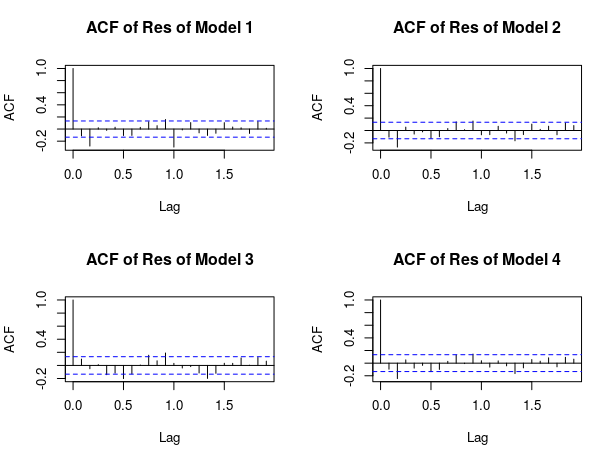
\includegraphics[scale=1.2]{1e1}
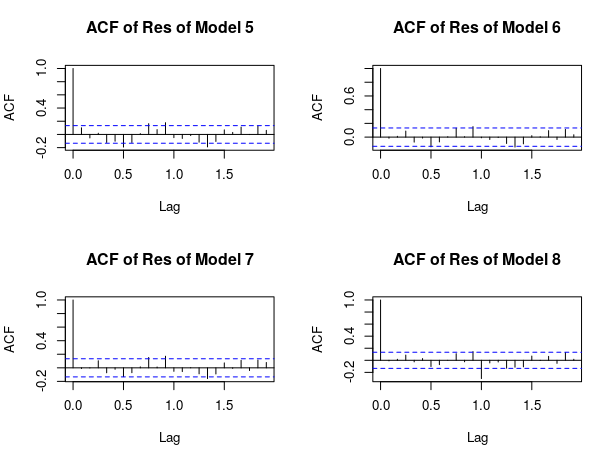
\includegraphics[scale=1.2]{1e2}
\end{center}
Here I decide to remove Model 1, 2, 4, and 8 as they either have early significant lags or a significant lag at the seasonal step thus indicating that they did not do an adequate of correctly modeling the data. 
\\\\
Next, I compare the p-values of the coefficients of the remaining subset of models to check whether they are significant or not. I select against those whose model coefficients are all non-significant. Using this condition of ALL, I am unable to erase any of the models from consideration.
\begin{center}
Model 3: $SARIMA(0,1,1)(0,1,1)_1 2$ \\
Model 5: $SARIMA(0,1,1)(1,1,0)_1 2$ \\
Model 6: $SARIMA(1,1,1)(1,1,1)_1 2$ \\
Model 7: $SARIMA(1,1,1)(1,1,0)_1 2$ 
\end{center}
Above are my remaining models.
\\\\
f.
\textbf{Figure 1}
\begin{table}[h]
\centering
\begin{tabular}{cccc}
Model   & AIC     & $\hat{\sigma^2}$ & RMSE     \\
$SARIMA(0,1,1)(0,1,1)_1 2$ & 1420.42 & 61.34                              & 17392.2  \\
$SARIMA(0,1,1)(1,1,0)_1 2$ & 1426.52 & 63.54                              & 21242.92 \\
$SARIMA(1,1,1)(1,1,1)_1 2$ & 1415.5 & 58.38
& 11296.16 \\
$SARIMA(1,1,1)(1,1,0)_1 2$ & 1422.09 & 61.42                              & 17310.1 
\end{tabular}
\end{table}
.
\\\\
g.
\\\\
According to RMSE in figure 1, I select $SARIMA(1,1,1)(1,1,1)_1 2$. This model has the following equation:
$$ (1 - 0.2078 B^{12})(1 - 0.2840 B)(1 - B^{12})(1 - B)y_t = (1 + (-0.6175)B^{12})(1 + (-0.8338)B)w_t $$
According to lowest AIC, I will select $SARIMA(1,1,1)(1,1,1)_1 2$ since it has the lowest value in comparison to the other models.
\\\\
According to $\hat{\sigma^2}$, I will select $SARIMA(1,1,1)(1,1,1)_1 2$ since it has the lowest value in comparison to the other models.
\\\\
h. After looking the ACF's of the residuals of the selected model, we know they all are statistically sound as they produce white noise. Also, we know that each of these models have at least one statistically significant coefficent, as also discovered in part Compared to the other statistics, RMSE takes precedence over the others so I will select $SARIMA(1,1,1)(1,1,1)_1 2$ as my most statistically valid model. Here is the forecasting model equation of that model in polynomial form:
$$ (1 - 0.2078 B^{12})(1 - 0.2840 B)(1 - B^{12})(1 - B)y_t = (1 + (-0.6175)B^{12})(1 + (-0.8338)B)w_t $$
Lastly, here is the plot of my forecast with the confidence interval of the forecast indicated in red. (I used the window function to get a better close up of the forecast)
\begin{center}
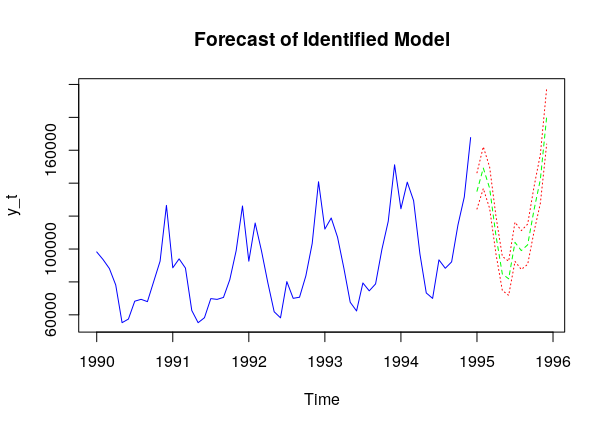
\includegraphics[scale=1]{1h}
\end{center}

\end{document}
